\documentclass{book}

\usepackage[spanish]{babel}
\usepackage[utf8]{inputenc}

\usepackage{graphicx}
\usepackage{lipsum}
\usepackage{microtype}

\usepackage[T1]{fontenc}
\usepackage{lmodern}

\usepackage[pdftex]{hyperref}

\hypersetup{pdfauthor={J. S. Castellanos-Durán},pdftitle={RECANEWS Volumen 3 - Marzo 2015},colorlinks,linkcolor=black,urlcolor=blue}

\usepackage[paperwidth=210mm, paperheight=297mm, textwidth=160mm, textheight=240mm, bindingoffset=1cm]{geometry}


% obliczenie szerokości lewego marginesu
\usepackage{calc}
\newlength{\lmargin}
\setlength{\lmargin}{1in + \hoffset + \oddsidemargin}

\usepackage{flowfram}

\usepackage{color}

\usepackage{tikz}
\usepackage{anyfontsize}

% definicja ramek typu flow umieszczonych na stonie 1
\newflowframe[1]{8cm}{24\baselineskip}{-.50cm}{0\baselineskip}[frame1-1a]
\newflowframe[1]{8cm}{23\baselineskip}{8.5cm}{0\baselineskip}[frame1-2b]
%\newflowframe[1]{5cm}{27\baselineskip}{11cm}{0\baselineskip}[frame1-3c]

%definicja ramek statycznych wstawianych na stronie 1
\newstaticframe[1]{\paperwidth}{14cm}{-\lmargin}{12.5cm}[frameS-1a]
\newstaticframe[1]{14cm}{7\baselineskip}{0cm}{45\baselineskip}[frameS-1b]

%definicja ramki dymamicznej wstawiania na stonie nieparzystej
\newdynamicframe[odd]{2cm}{2cm}{-\lmargin}{6cm}[frameD-1a]
%definicja ramki dymamicznej wstawiania na stonie parzystej
\newdynamicframe[even]{2cm}{2cm}{\textwidth+\lmargin-2cm}{6cm}[frameD-1b]

% definicja ramek typu flow na kolejnych stronach
\newflowframe[>1]{8cm}{57\baselineskip}{-.50cm}{0\baselineskip}[frame2-1a]
\newflowframe[>1]{8cm}{57\baselineskip}{8.5cm}{0\baselineskip}[frame2-2a]
%\newflowframe[>1]{5cm}{57\baselineskip}{11cm}{0\baselineskip}[frame2-3a]

\definecolor{green}{rgb}{0.6,0.8,0.1}

\title{RECANEWS Volumen 3 - Marzo 2015}
\author{J. Sebastián Castellanos Durán}
\date{\relax}

\begin{document}

\pagestyle{empty}

% wstawienie numerów stron w ramki dynamiczne frameD-1a i frameD-1b
\begin{dynamiccontents*}{frameD-1a}
\begin{tikzpicture}
\draw(0,0) node [fill=orange, minimum width=2cm, minimum height=2cm]{
{\sffamily\bfseries\Huge\color{white}\thepage}
};
\end{tikzpicture}
\end{dynamiccontents*}

\begin{dynamiccontents*}{frameD-1b}
\begin{tikzpicture}
\draw(0,0) node [fill=orange, minimum width=2cm, minimum height=2cm]{
{\sffamily \bfseries\Huge\color{white}\thepage}
};
\end{tikzpicture}
\end{dynamiccontents*}


% wstawienie grafiki w ramkię statyczną frameS-1a
\begin{staticcontents*}{frameS-1a}
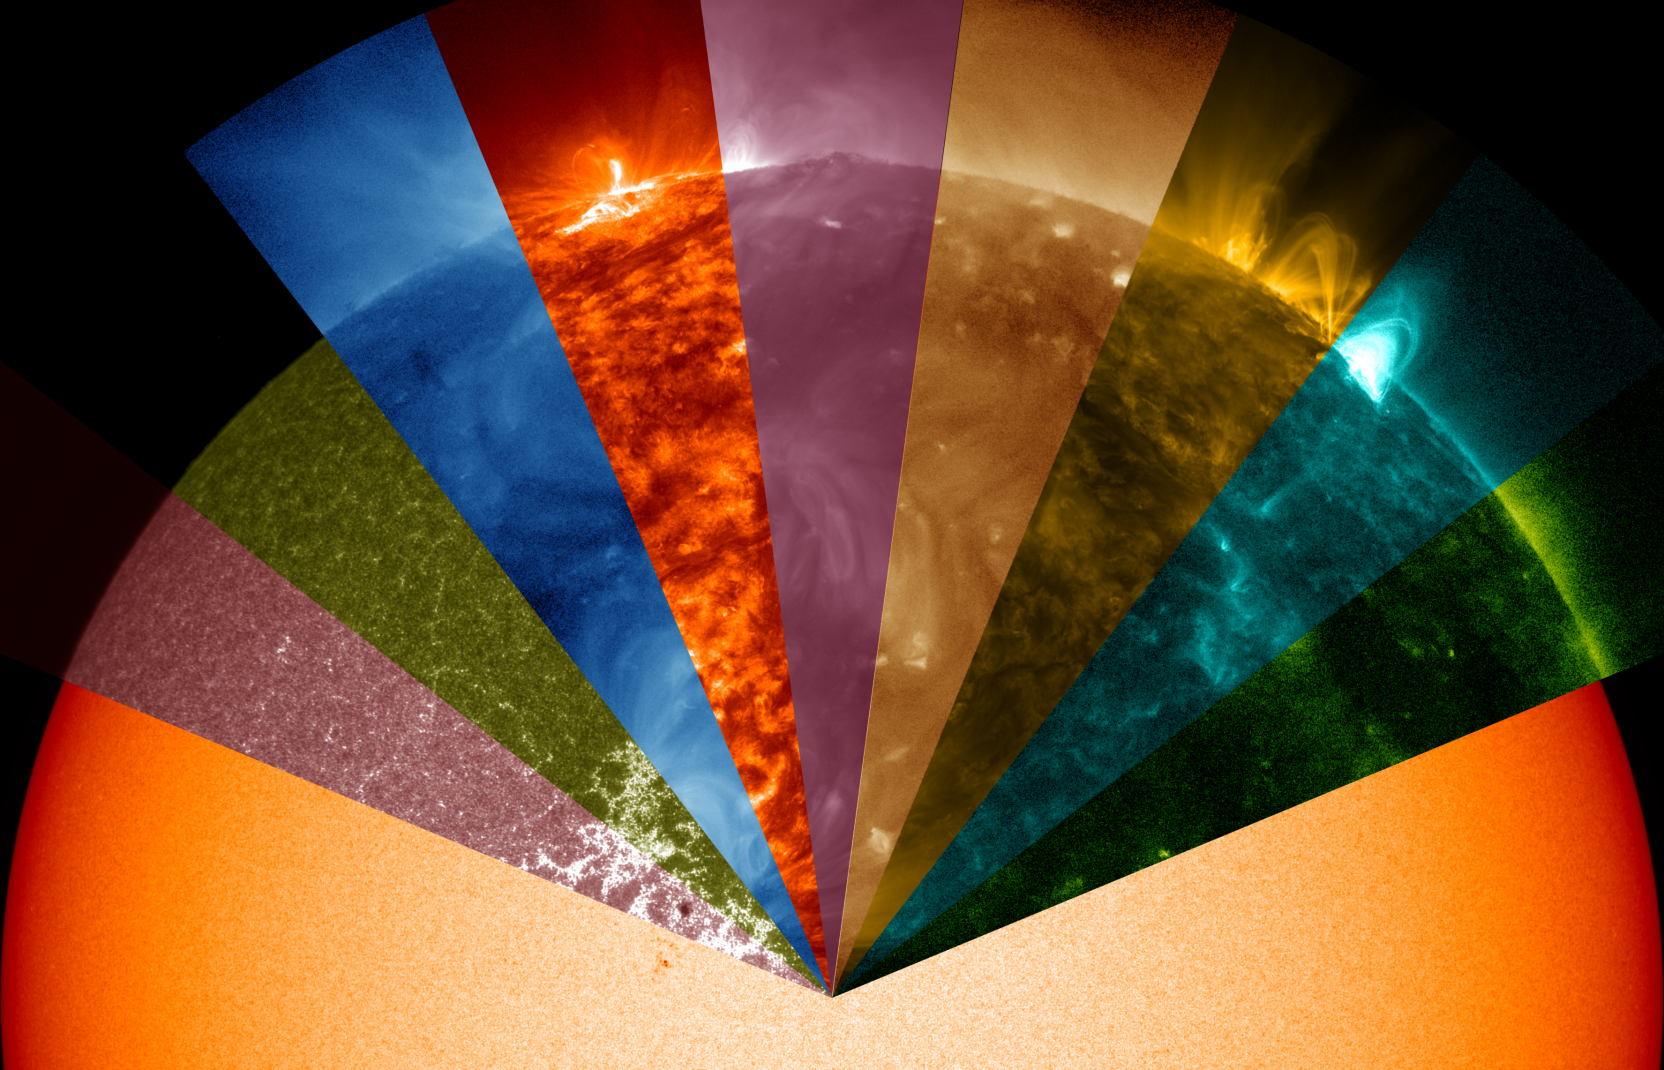
\includegraphics[width=1.0\textwidth]{fig22.png}
\end{staticcontents*}

% wypełnienie tekstem ramki statycznej frameS-1b
\begin{staticcontents*}{frameS-1b}
\begin{tikzpicture}
\draw(0,0) node [fill=white, text width=13cm, inner sep=5mm, opacity=0.7]{
\large\sffamily
{\fontsize{70}{30}\selectfont {\color{black} RECANEWS}}\\


{\fontsize{30}{30}\selectfont {\color{black} Volumen 3}}\\
\begin{flushright}
{\fontsize{30}{30}\selectfont {\color{black} Marzo 2015}}
\end{flushright}
};
\end{tikzpicture}
\end{staticcontents*}


\tableofcontents{}
% wlanie tekstu do wszystkich ramek typu flow




\renewcommand\thesection{\arabic{section}}
\renewcommand\thesubsection{\arabic{subsection}}

%*********************************************
\addcontentsline{toc}{section}{Noticias Astronomía y ciencias del espacio en Colombia}
\section*{Noticias Astronomía y ciencias del espacio en Colombia}
%*********************************************
%*********************************************
\subsection{La UIS en la colaboración Auger}
%*********************************************
Al occidente de Argentina el Pierre Auger Cosmic Ray Observatory estudia las partículas muy energéticas provenientes del Universo, las cuales por su interacción con la atmósfera terrestre presentan grandes cascadas de partículas secundarias y nos permiten estudiar los rayos cósmicos. Los rayos cósmicos de bajas y moderadas energías están bien entendidos; sin embargo, aquellos con energías extremadamente altas permaneces aún un misterio. Detectando y estudiando estas partículas el Observatorio Auger está abordando los enigmas sobre su origen y existencia.

La colaboración Pierre Auger Collaboration include más de 500 científicos provenientes de Argentina, Austrañia, Brasil, Croacia, República Checa, Francia, Alemania, Italia, México, Holanda, Polonia, Portugal, Rumania, Eslovenia, España, el Reino Unido y U.S.A. Recientemente, y para la alegría de la comunidad de astronomía y altas partículas en Colombia, nuestro país es nuevo miembro de esta colaboración por la Universidad Industrial de Santander (UIS), Bucaramanga. \\


%*********************************************
\subsection{Publicación - Juan D. Soler}
%*********************************************

El astrónomo Juan Diego Soler que se encuentra actualmente en el Instituto de Astrofísica - Paris,  escribió dentro de la colaboración Planck un artículo el cual fue recientemente enviado a la revista A\&A recientemente.
En este artículo se estudia del rol de campo magnético en la formación de estructuras en el ISM a partir de las observaciones de la emisión térmica polarizada del polvo interestelar que hizo el observatorio espacial Planck. Los comentario sobre este artículo son bienvenidos.

La versión de este artículo se puede encontrar en\\
 
\url{http://arxiv.org/abs/1502.04123}

%*********************************************
\subsection{Nuevo programa radial sobre Astronomía en Colombia}
%*********************************************

\textbf{Astronomía al Aire}, una cita con el Cielo La noche, los astros, el universo han ejercido una fascinación persistente en hombres y mujeres a través de los tiempos. Astronomía al Aire busca apoyarse en esa fascinaciónpara contribuir a crear una cultura científica. Crear curiosidad por el diverso mundo de la astrofísica, de lo que sabemos, de lo que ignoramos.\\
\\
Una serie de micros radiales usa el poder de penetración de la radio para seducir al oyente.  Todos los días a través de  UIS AM- 670KHz a las 7:00 a.m. 12:30 p.m y 5:30 p.m podrán escuchar un apasionante tema semanal. Esta semana se conversa sobre los agujeros negros, el triunfo de la gravedad.\\
\\
Un blog http://halley.uis.edu.co/aire/ les da permanencia y los complementa preservando el audio y planteando preguntas.  En el blog el visitante puede puede oír los micros, leer los textos y formular comentarios, preguntas e inquietudes que serán respondidas en línea, a través @AstroAlAire y astronomia.al.aire@uis.edu.co .\\
\\
Un programa radial más largo con invitados, permitirá ampliar los temas y mantener el interés de los oyentes..\\
\\
Astronomía al Aire deriva de los esfuerzos que el Grupo Halley ha venido desarrollando a lo largo de varios lustros en la promoción de la Astronomía en el Nororiente colombiano.\\
\\
Es posible gracias al profesionalismo de TeleUIS Comunicaciones, al respaldo entusiasta de la Vicerrectoría de Investigación de la Universidad Industrial de Santander y al apoyo irrestricto de la Escuela de Física. Está coordinada por Héctor Rago y Luis Núnez.



%*********************************************
\subsection{Nuevo docente en astronomía - ECCI}
%*********************************************

El Dr. Oscar Leonardo Ramírez Suárez fue contratado desde Enero como Docente Investigador en la Universidad ECCI. Es Físico de la U. Nacional, donde hizo su pregrado en Física Nuclear en el Centro Internacional de Física. Luego estudió su MSc en el Instituto Balseiro en Argentina en Física de Altas Energías, becado por el ICTP. Posteriormente hizo su doctorado en la U. Libre de Bruselas en Física Nuclear. Su área principal de investigación es en modelos teóricos de reacciones nucleares aplicados a astrofísica. Tiene colaboraciones activas con la ULB (Bélgica) y el CIF (Colombia). En la UECCI trabajará con el grupo de Ciencias Básicas conformado por Germán Chaparro, Oscar Restrepo y co-investigadores, apoyando también las líneas de investigación de Radioastronomía y Astroestadística.

\begin{flushright}
Germán Chaparro Molano, PhD
\end{flushright}


%*********************************************
\subsection{Charlas en Spacio - Marzo}
%*********************************************
El Seminario de Astronomía y ciencias del espacio (Spacio) se lleva acabo en el Planetario de Bogotá todos los Sábados de 4pm a 6pm. Las presentaciones para el mes de Marzo son 

\begin{description}
\item[Marzo 7 - 4:00pm:] Influencia de rotación y outflows en Lyman Alpha Emitters\\
Maria Camila Remolina\\
Uniandes.
\item[Marzo 7 - 5:15pm:] Modelos de Formación Estelar en Simulaciones de Galaxias\\
Luis Fernando Quiroga\\
Universidad de Antioquia.
\item[Marzo 14 - 4:00pm:] ¿Una secuencia principal de galaxias?\\ 
Juan Rafael Martinez Galarza\\ 
Harvard-Smithsonian Center for Astrophysics. 
\item[Marzo 14 - 5:15pm:] Magneto no es un héroe: campos magnéticos y la formación de estrellas\\ 
Juan Diego Soler\\
Instituto de Astrofísica Paris.   
\item[Marzo 21 - 4:00pm:] Geología y Astrobiología\\ 
Julian Corzo\\  
Universidad Nacional de Colombia
\item[Marzo 21 - 5:15pm:] Sociología y Materia Oscura\\
Paola Casteño\\ 
UniAndes  
\item[Marzo 28 - 4:00pm:] Las galaxias satélite y su extraña y su extraña distribución espacial\\
Veronica Arias\\
UniAndes.
\item[Marzo 28 - 5:15pm:] Asociaciones de Galaxias Enanas en el Grupo Local\\
Juan Nicolas Garavito\\
UniAndes 
\end{description}

\noindent La programación completa puede ser descargada por medio de los siguientes links:

\begin{itemize}
\item \url{http://goo.gl/i0aSCw}
\item \url{http://goo.gl/kQmbHc}
\end{itemize}

%*********************************************
\subsection{COCOA Libro de resumenes}
%*********************************************

COCOA Libro de resumenes

\subsection{1st workshop on Current Challenges in Cosmology: Inflation and the Origin of CMB anomalies.\\ Mayo 18 - 22, 2015 Cali, Colombia}
The Workshop is intended to gather leading experts in theoretical Cosmology to share knowledge, discuss new theoretical developments in inflationary cosmology and ultimately elucidate the puzzle of CMB anomalies. 
\textbf{Main topics}
\begin{itemize}
\item Statistical anisotropy and anisotropic expansion
\item Primordial magnetic fields
\item Parity violation and polarization in the CMB
\item Effective field theory of inflation
\item Anisotropic non-gaussianity
\item CMB data analysis
\item Primordial Gravitational  Waves
\item Galileons and Horndeski theories
\end{itemize}
\par
\noindent Invited Speakers:\\
\\
Konstantinos Dimopoulos (Lancaster University),	David F. Mota (University of Oslo), Maresuke Shiriashi (Università degli Studi di Padova), Patrick Peter
(Institut d’Astrophysique de Paris), Azadeh Maleknejad (Institute for Research in Fundamental Sciences), Marco Peloso (University of Minnesota), Lorenzo Sorbo (University of Massachusetts), Thiago S. Pereira (Universidade Estadual de Londrina), Leonardo Senatore* (Stanford University), Mindaugas Karciauskas (Helsinki University), Martin Bucher (University Paris 7 Diderot).\\
\\
Más información

\begin{center}
\url{cosmology.univalle.edu.co/index.php/home}
\end{center}

Contacto:\\
\begin{flushright}
\url{juanpbeltran@uan.edu.co}\\
\url{cesar.valenzuela@correounivalle.edu.co}\\
\url{yeinzon.rodriguez@uan.edu.co}
\end{flushright}

%*********************************************
\subsection{COCOA Publicación memorias}
%*********************************************

COCOA Publicación memorias

%*********************************************
\subsection{2do Science Hack Day bogotá - Pre inscripciones abiertas}
%*********************************************

Ya están abiertas las preinscripciones para el Segundo Science Hack Day Bogotá, que tendrá lugar del 21 al 22 de Marzo de 2015 en el Planetario de Bogotá. No importa que seas artista, diseñador, ingeniera, matemático, filósofa o simplemente un entusiasta de la ciencia, el Science Hack Day es el lugar para ti.\\
\\
Más información
\begin{center}
\url{http://bogota.sciencehackday.org/}
\end{center}

%*********************************************
\addcontentsline{toc}{section}{Escuelas}
                   \section*{Escuelas}
%*********************************************

%*********************************************
\subsection{XXIV Verano en el Observatorio 2015 - Deadline 20 de Abril}
%*********************************************
El Instituto de Astronomía de la UNAM te invita al XXIV Verano en el Observatorio, a realizarse del 1 al 26 de Junio en Ensenada, Baja California, México

\begin{description}
\item[SOLICITUDES:] 1 de Febrero al 20 de Abril

\item[RESULTADOS:] 22 de Abril

\item[Objetivo:]
\end{description}
Proveer un conocimiento teórico-práctico de diversos aspectos de la astronomía actual, así como un acercamiento a la investigación científica.
\begin{description}
\item[Información:]
\end{description}
El curso esta dirigido a estudiantes de licenciatura en física o en ciencias afines que estén interesados en adquirir un conocimiento amplio de la astrofísica actual y de las técnicas observacionales mas usadas en el óptico e infrarrojo.\\
\\
Los estudiantes seleccionados tendrán la oportunidad de participar con un investigador en el desarrollo de un proyecto, el cual se presentara al final del curso. ademas podrán trabajar algunas noches con los telescopios del observatorio astronómico nacional.\\

Más información 
\begin{center}
\url{http://www.astrosen.unam.mx/~verano/}
\end{center}
\begin{flushright}
Katherine Mafla
\end{flushright}

%*********************************************
\subsection{Undergraduate Astronomy Research Scholarship - Yale University}
%*********************************************

The Yale University Astronomy Department is pleased to invite applications for the second annual Hoffleit Undergraduate Astronomy Research Scholarship. This program serves as an opportunity for keen undergraduates in STEM fields with a strong interest in pursuing astronomy to spend 6-8 weeks performing research with Yale astronomers. Research topics cover a wide range, from the characterization and discovery of exoplanets, the study of the Sun and stars, to the origin and evolution of small and large galaxies. Yale’s astronomy department is located in New Haven, CT, near historic downtown and the East Rock neighborhood. New Haven is a vibrant city in the summertime; home to the Arts and Ideas festival, as well as many cafes and restaurants. The undergraduate students will be housed together in the beautiful campus residential colleges where they will have the opportunity to interact with undergraduate scholars from other departments.\\
\\
The program encourages undergraduates from all nationalities to apply, particularly those with a strong desire to continue to graduate school.\\
\\
To apply or find out more, visit\\ \url{http://goo.gl/sYbj6H}\\
\\
The fellowship is named in honor of Dr. E. Dorrit Hoffleit, was a senior research astronomer at Yale for more than fifty years in the University’s Department of Astronomy.


%*********************************************
\addcontentsline{toc}{section}{Programas de posgrados}
\section*{Programas de posgrados}
%*********************************************


%*********************************************
\subsection{Posgrados en la UniAndes}
%*********************************************

Ya están abiertas las inscripciones al posgrado (Maestría, Doctorado) de Física en Uniandes donde el grupo de astrofísica puede ofrecer temas de investigación. La fecha límite es el 28 de Abril.\\
\\
Este año aparte de la posibilidad de apoyo financiero a través de asistencias graduadas también hay becas de Colciencias (para personas que ya tengan una maestría).\\

Si les interesa saber más sobre los detalles pueden escribirme un correo a \url{je.forero@uniandes.edu.co}. Además, el 4 de marzo habrá una charla informativa sobre posgrados en Uniandes (programas, fuentes de financiación, etc).\\

Los interesados pueden inscribirse en:\\

\begin{center}
\url{http://goo.gl/UfPi3q}
\end{center}

\begin{flushright}
Jaime Forero
\end{flushright}


\subsection{Inscripciones Abiertas Maestría en Astronomía en el Observatorio\\ Astronómico Nacional y en Física\\ Universidad Nacional}

\begin{itemize}
\item Pago de derechos de inscripción \\
\textbf{HASTA EL 13 DE ABRIL DE 2015}
\item Formalización de la inscripción\\
\textbf{DESDE EL 9 DE FEBRERO}\\
\textbf{HASTA EL 13 DE ABRIL DE 2015}
\end{itemize}

Mas Informacion:
\begin{center}
\url{http://admisiones.unal.edu.co/}
\end{center}


\begin{flushright}
J. Sebastian Castellanos Duran
\end{flushright}



%*********************************************
%*********************************************
\addcontentsline{toc}{section}{Congresos y eventos}
\section*{Congresos y eventos}
%*********************************************

\subsection{EWASS 2015\\ Deadline: 10 March 2015}

The European Week of Astronomy and Space Science (EWASS, formerly JENAM) is the annual meeting of the European Astronomical Society (EAS). With more than 20 years of tradition, it has imposed itself as the largest conference for European astronomy. In addition to plenary sessions and the award of prestigious prizes, the conference hosts many symposia held in parallel, as well as special sessions and meetings.\\

\noindent The EAS together with one of its affiliated societies, organises the annual EWASS conference to enhance its links with national communities, to broaden connections between individual members and to promote European networks.\\

\noindent EWASS 2015 is held for the first time in Tenerife, Spain and is expected to welcome over 600 astrophysicists from all over Europe and even beyond.\\

\noindent Más información:
\begin{center}
\url{ http://eas.unige.ch/EWASS2015/index.jsp}
\end{center}


%*********************************************
\addcontentsline{toc}{section}{Opinión}
\section*{Opinión}
%*********************************************

%*********************************************
\subsection{¿Estás pensando en hacer un Ph.D?}
%*********************************************

Si estás pensando en hacer un Ph.D en ciencias este artículo es para ti. Un aparte dice:\\

\textit{``... we have a field of understandably disgruntled young people with PhDs but no realistic prospect of ever earning a settled living working in the field they have prepared for. This problem has worsened considerably in recent  years as the number of postdoctoral positions has almost halved since 2006. New PhDs have to battle it out with existing postdoctoral researchers for the meagre supply of suitable jobs. It’s a terrible situation.''}\\

Artículo completo:
\begin{center}
\url{http://goo.gl/QTTsjN}
\end{center}



%*********************************************
\addcontentsline{toc}{section}{¿Cómo publicar en RECANEWS?}
\section*{¿Cómo publicar en RECANEWS?}
%*********************************************

Para publicar en RECANEWS se debe enviar un correo a reca.news@gmail.com con las siguientes especificaciones:
\begin{description}
\item[Correo:]\url{reca.news@gmail.com}
\item[Asunto:]Título de la publicación
\item[Contenido:]Contenido de la publicación\\
Persona encargada (Opcional)\\
Correo de la persona encargada (Opcional)
\end{description}
  
%*********************************************
\addcontentsline{toc}{section}{Repositorio de RECANEWS}
\section*{Repositorio de RECANEWS}
%*********************************************

Repositorio: \url{https://github.com/recanews}\\



%*********************************************
\addcontentsline{toc}{section}{Contacto del RECA}
\section*{Contacto del RECA:}
%*********************************************

\begin{description}
\item[Correo RECA:]\url{reca.astronomia@gmail.com}
\item[Facebook:] \url{https://www.facebook.com/RECAstronomia}
\item[Google$+$:] \url{http://goo.gl/P0DEf4}
\item[Twitter:] \url{https://twitter.com/RECAstronomia}
\item[Pagina Web:] \url{http://goo.gl/Fl4zQP}
\end{description}


%*********************************************
\addcontentsline{toc}{section}{Representantes de RECA en las regiones}
\section*{Representantes de RECA en las regiones}
%*********************************************
\begin{description}
\item[Medellín:]Malory Agudelo Vásquez\\
\url{magudelov@gmail.com}\\ \url{magudelov@fisica.udea.edu.co}
\item[Pereira:]Luisa Fernanda Cardona\\ \url{luisferncardona@utp.edu.co}
\item[Pasto:]Katherine Mafla Oliva\\
\url{skmofis13@gmail.com}
\item[Cali:]Daniel Santacruz\\
\url{santacruz121@gmail.com}
\item[Bogotá:]Maria Camila Remolina Gutierrez\\
\url{mc.remolina197@uniandes.edu.co}\\

Andres Felipe Ramos Padilla\\
\url{andresrp25@gmail.com}\\

Juan David Jimenez Nieto\\
\url{jdjimenezn@correo.udistrital.edu.co}
\end{description}


%*********************************************
\addcontentsline{toc}{section}{Editor RECANEWS}
			\section*{Editor RECANEWS}
%********************************************
  
\begin{flushright}
J. Sebastián Castellanos-Durán\\
\url{jsebastian405@gmail.com}
\end{flushright}
\begin{flushright}
Cualquier comentario por favor escribir al correo  \url{reca.news@gmail.com}\\
Marzo 2015
\end{flushright}


\end{document}


